\documentclass[justified,nobib]{tufte-handout}
\usepackage{microtype}
\usepackage[english]{babel}
\usepackage{inputenc}
\usepackage{graphicx}
\usepackage{amsthm}
\usepackage[ruled,vlined]{algorithm2e}
\usepackage{algorithmic} 
\usepackage{amsmath}
\usepackage{amsmath}
\usepackage{amssymb}
\usepackage{listings}
\usepackage{hyperref}
\usepackage{bm}
\lstdefinestyle{mystyle}{
    % backgroundcolor=\color{backcolour},   
    commentstyle=\color{magenta},
    % keywordstyle=\color{magenta},
    numberstyle=\tiny\color{gray},
    % stringstyle=\color{codepurple},
    basicstyle=\ttfamily\small,
    breakatwhitespace=false,         
    breaklines=true,                 
    captionpos=b,                    
    keepspaces=true,                 
    numbers=left,                    
    numbersep=5pt,                  
    showspaces=false,                
    showstringspaces=false,
    showtabs=false,                  
    tabsize=2
}
\lstset{style=mystyle}


\usepackage[square,sort,comma,numbers]{natbib}
\title{ece453 - Final Project}
\author{Armaan Kohli}
\date{\today}
\begin{document}
\begin{fullwidth}
\selectlanguage{English}
{
  \noindent\fontsize{12pt}{20pt}\selectfont\textbf{Final Project: GPU Accelerated Support Vector Machines via Quadratic Programming}
  \newline
  \fontsize{12pt}{18pt}\selectfont
  {Armaan Kohli - \scshape ece}453 Advanced Computer Architecture \\Spring 2020\\
}
\raggedright
\raggedbottom
\section{Remarks}
\paragraph{} We implemented a fast support vector machine (SVM) classifier that leverages GPU architecture to achieve performance gains for large datasets. Specifically, our project formulates a SVM classifier as a quadratic program, which we can solve using the alternating direction method of multipliers (ADMM) with either LDL factorisation on the CPU or preconditioned conjugate gradient (PCG) on the GPU. Our project is an extension of the the \texttt{osqp} API \cite{osqp}, having added additional tools for SVM problem generation and linear system solving using PCG and CUDA to target an Nvidia Jetson Nano. We compare the results of our GPU implementation to the benchmarks provided by \texttt{osqp}.

\section{Support Vector Machines}
\paragraph{}

The support vector machine (SVM) is an example of a convex optimization problem w/ quadratic criteria. SVM is a technique for classifying data that may not be linearly separable. This is accomplished by performing a linear classification problem in a higher dimensional feature space where the data is linearly separable. 
\end{fullwidth}
\begin{marginfigure}[3in]
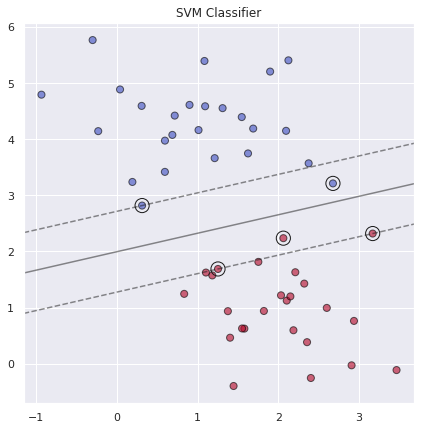
\includegraphics[scale=.4]{./media/svm.png}
\caption{An illustrative example of an SVM classifier. Most of the construction of the SVM section is based on \textit{The Elements of Statistical Learning} \cite{stat}.}
\label{fig:plot}
\end{marginfigure}

First, let's assume we have $N$ tuples, $(x_i, y_i)$, where $x_i \in R^m$ represent feature vectors, and $y_i$ represents the true class, $y_i \in \{-1, 1\}$. For instance, in the Fig \ref{fig:plot}, the blue dots correspond to $x_i$ from $y_i = -1$, and the red dots correspond to features from $y_i = 1$. Let's also assume we've already done some kind of projection into a space where the classes are linearly separable. 

Now, we only have access to each value of $x_i$, the class they belong to, the corresponding $y_i$, is unknown. 
Let's define a hyperplane by: 

\begin{equation}
\{ x: f(x) = x^T\beta + 1 = 0 \}
\end{equation}

A classification rule induced by this hyperplane $f(x)$ is:
\begin{equation}
G(x) = sign[x^T\beta +1 ]
\end{equation}

Since we are in a space where the classes are linearly separable, we can find a function $f(x) = x^T\beta + 1 $ with $y_if(x_i) > 0 \; \; \forall \; i$. Hence, we are able to find a hyperplane that creates the largest margin between the two classes. This is what the SVM accomplishes. 

\begin{fullwidth}

The circled points on the dotted lines are the so-called support vectors. The points between the dashed line and the decision boundary are within the margin. The SVM seeks to find the hyperplane that creates the largest margin, subject to the constraint to minimize the total distance of points on the wrong side of the margin.

We can formulate an SVM as a quadratic program using the method described in \citep{stat}. In this form, we can use an algorithm called alternating direction method of multipliers (ADMM). 
%We can solve classification problems more efficiently by re-writing the problem as one from convex optimization. Traditionally, the SVM is captured by the following:
%\begin{gather*}
% \underset{\beta}{\operatorname{max}} M \\
%\text{subject to:} \; \;
%y_i(x_i^T\beta + 1) \geq M, i=1, \dots N 
%\end{gather*}
%
%Where, $M$ denotes the width of the margin. We can re-write this has
%\begin{gather*}
%\underset{\beta}{\operatorname{min}} \lVert \beta \rVert \\
%\text{subject to: } \; \; y_i(x_i^T\beta + 1) \geq 1, i=1, \dots N,\;\;\;\; \text{where}\;\;\; M = 1/\lVert \beta \rVert  
%\end{gather*}
%
%Suppose that the classes overlap in feature space, ie the two classes aren't perfectly linearly separable. Then, we can modify our constraint to still maximize $M$, but allow for points to be on the wrong side of the margin. These points are called slack variables (these are the circle points that aren't on the dotted lines). So, we need to modify our constraint to:
%
%\begin{equation}
%y_i(x_i^T\beta + 1) \geq M(1-\xi_i), i=1, \dots N
%\end{equation}
%where $\xi_i$ are slack variables. This allows us to re-write our problem as:
%\begin{equation}
%\underset{\beta}{\operatorname{min}} \lVert \beta \rVert \;\; \\
%\text{subject to: }
% \begin{cases} 
%      y_i(x_i^T\beta + 1) \geq 1 - \xi_1 \forall i \\ \\
%      \xi_i > 0, \sum \xi_i \leq C, \text{where $C$ is some constant. } \\     
%   \end{cases}
%\end{equation} 
%Now, we can formulate Eq. 4 as a convex quadratic program using Lagrange Multipliers. We can re-write Eq. 4 as 
%\begin{equation}
%\begin{split}
%& \underset{\beta} {\operatorname{min}} \frac{1}{2}||\beta||^2 + C \sum_{i=1}^{N} \xi_i \\ 
%& \text{subject to:} \; \; \xi_i \geq 0, \; \;y_i(x_i^T\beta + 1) \geq 1 - \xi_i \; \forall i 
%\end{split}
%\end{equation}
%The Lagrange (primal) function is:
%\begin{equation}
%L_P = \frac{1}{2}||\beta||^2 + C \sum_{i=1}^{N} \xi_i - \sum_{i=1}^{N}
% \alpha_i \left[ y_i \left( x_i ^T \beta +1 \right) - (1-\xi_i)\right] - \sum_{i=1}^{N} \mu_i \xi_i
%\end{equation}
%We then minimize the Lagrange function with respect to $\beta$ and $\xi_i$ by taking the derivative and setting it equal to zero. This yields the following conditions
%\begin{equation}
%\beta = \sum_{i=1}^{N} \alpha_i y_i x_i
%\end{equation}
%\begin{equation}
%0 = \sum_{i=1}^{N} \alpha_i y_i
%\end{equation}
%\begin{equation}
%\alpha_i = C - \mu_i, \;\;\; \forall i
%\end{equation}
%Then, we can substitute these relationships into the Lagrange primal function to compute the corresponding dual objective, which is easier to minimize.
%\begin{equation}
%L_D = \sum_{i=1}^{N} alpha_i - \frac{1}{2}\sum_{i=1}^{N} \sum_{j=1}^{N} \alpha_i \alpha_j y_i y_j x_i^T x_j
%\end{equation}
%Which gives a lower bound to our original objective, Eq. 5.To maximize $L_D$, we must also a set of additional constraints called the Karush-Kuhn-Tucker conditions. 
%\begin{equation}
%\alpha_i [y_i (x_i^T \beta + 1) - (1-\xi_i)] = 0
%\end{equation}
%\begin{equation}
%mu_i\xi_i = 0
%\end{equation}
%\begin{equation}
%y_i(x_i^T\beta + 1) - (1-\xi_i) \geq 0
%\end{equation}
%These equations fully define a primal and dual problem, which allows us to use ADMM to solve.

% The main contribution of the \texttt{osqp} paper is a simplification to the ADMM problem. The algorithm they use is below





 
\section{Implementation Details}
\paragraph{}
The \texttt{osqp} paper presents an two new ways of solving ADMM, a direct method an indirect method. The algorithm in full-form is presented below:
\begin{algorithm}[htp][
\SetKwInOut{Input}{input}\SetKwInOut{Output}{output} 
\SetAlgoLined
\textit{given:}
 $x^0, z^0, y^0 \; \textit{and parameters} \;\rho >0, \; \sigma >0, \; \alpha \in [0,2]$
 \\ \While{\textit{not terminated}}{
 ${(\tilde{x}^{k+1}, v^{k+1}) \leftarrow \begin{bmatrix}
P+\sigma I & A^T\\
A & -\rho^{-1}I  
\end{bmatrix}}
\begin{bmatrix}
\tilde{x}^{k+1}\\
v^{k+1}
\end{bmatrix}
= \begin{bmatrix}
\sigma x^k - q\\
z^k - \rho^{-1}y^k
\end{bmatrix}
$
\\
$\tilde{z}^{k+1} \leftarrow z^k + \rho^{-1}(v^{k+1} - y^k)$\\
$x^{k+1} \leftarrow \alpha\tilde{x}^{k+1} + (1-\alpha)x^k$ \\
$z^{k+1} \leftarrow \prod \left(\alpha\tilde{z}^{k+1}+(1-\alpha)z^k + \rho^{-1}y^k \right)$ \\
$y^{k+1} \leftarrow y^k + \rho(\alpha \tilde{z}^{k+1} + (1-\alpha)z^k - z^{k+1}$
 } \caption{ADMM algorithm as presented in \cite{osqp}}
\end{algorithm}
\paragraph{} Using this algorithm, we can very quickly compute solutions to SVM problems. However, there is one big issue with the algorithm, namely the matrix inversion step, which must be done every iterations until convergence. This is what we'll exploit to get performance gains. The CPU-based algorithm that \texttt{osqp} presents uses LDL matrix factorization to solve this linear system, called the KKT matrix. LDL factorization can be costly as the size of the problem increases, so for large datasets, we can leverage parallelism, and implement an indirect solver for this KKT matrix using PCG. As opposed to a direct method such as KKT, PCG can be efficiently parallelized. 

\subsection{Preconditioned Conjugate Gradient}
\paragraph{}
In cases where the number of datapoints or the dimensionality of the space is too large for LDL factorization to work effectively, we can instead use an indirect method for solving this KKT linear system. PCG was suggested as a solution in \cite{cuosqp}. This is accomplished by re-writing the KKT constraints as in the following form:
\begin{equation}
(P + \sigma I + A^TRA)\tilde{x}^{k+1} = \sigma x^k - q + A^T(Rz^k-y^k)
\end{equation}
Which can be solved using the PCG algorithm below. 
\begin{algorithm}[htp][
\SetKwInOut{Input}{input}\SetKwInOut{Output}{output} 
\SetAlgoLined
\textit{initialise:}
 $r^0 = Kx^0 -b, \; y^0 = M^{-1}r^0, \; p^0 = -y^0, \; k = 0 $
 \\ \While{$||r^k|| > \epsilon||b||$}{
$\alpha^k \leftarrow - \frac{\left(r^k\right)^Ty^k}{\left(p^k\right)^TKp^k} $\\
$x^{k+1} \leftarrow x^k + \alpha^k p^k$\\
$r^{k+1} \leftarrow r^k + \alpha^k K p^k$\\
$y^{k+1} \leftarrow M^{-1}r^{k+1}$\\
$\beta^{k+1} \leftarrow - \frac{\left(r^{k+1}\right)^Ty^{k+1}}{\left(r^k\right)^Ty^k} $\\
$p^{k+1} \leftarrow -y^{k+1} + \beta^{k+1}p^k$\\
$k \leftarrow k + 1 $
 } \caption{PCG algorithm as presented in \cite{cuosqp}}
\end{algorithm}\\

\subsection{GPU Optimizations}
\paragraph{}
In order to write an efficient GPU implementation of PCG, we used the following CUDA Toolkit libraries: \texttt{Thrust}, \texttt{cuBLAS} and \texttt{cuSPARSE}. \texttt{Thrust} provides a high-level interface for essential data parallel primitives, such as scan and sort operations. \texttt{cuBLAS} is a CUDA implementation of BLAS (Basic Linear Algebra Subprograms). We use only level-1 cuBLAS API functions that implement the inner product, axpyoperation, scalar-vector multiplication, and computation of norms. \texttt{cuSPARSE} is a CUDA library that contains a set of linear algebra subroutines for handling sparse matrices. Throughout the GPU codebase, we use a CSR format of sparse matricies, since that is the format that \texttt{cuSPARSE} uses. The rest of the \texttt{osqp} api uses CSC representation, so additional code was needed to perform conversion. 
\paragraph{} For the kernel functions, we used 64 elements per thread and 1024 threads per block. We found that this gave the best performance empirically, through a more thorough analysis or parameter search would be required to test for optimal settings.
 
 
\section{Results \& Discussion}
\paragraph{} In order to test the performance of our implementation, we generated random SVM problems of various dimensions and computed the run time. To create the CPU benchmarks, we use the CPU code provided by \texttt{osqp}. To test the GPU code, we used our own PCG implementation that we then interfaced with the \texttt{osqp} api. We generated the SVM problems using a simple \texttt{python} script and used the provided code generation tools provided by \texttt{osqp} to generate header files containing the data. Below in Fig. \ref{fig:cuosqp_results} is the performance of the SVM classifier according to the results from \citep{cuosqp}. 
\begin{figure}[h]
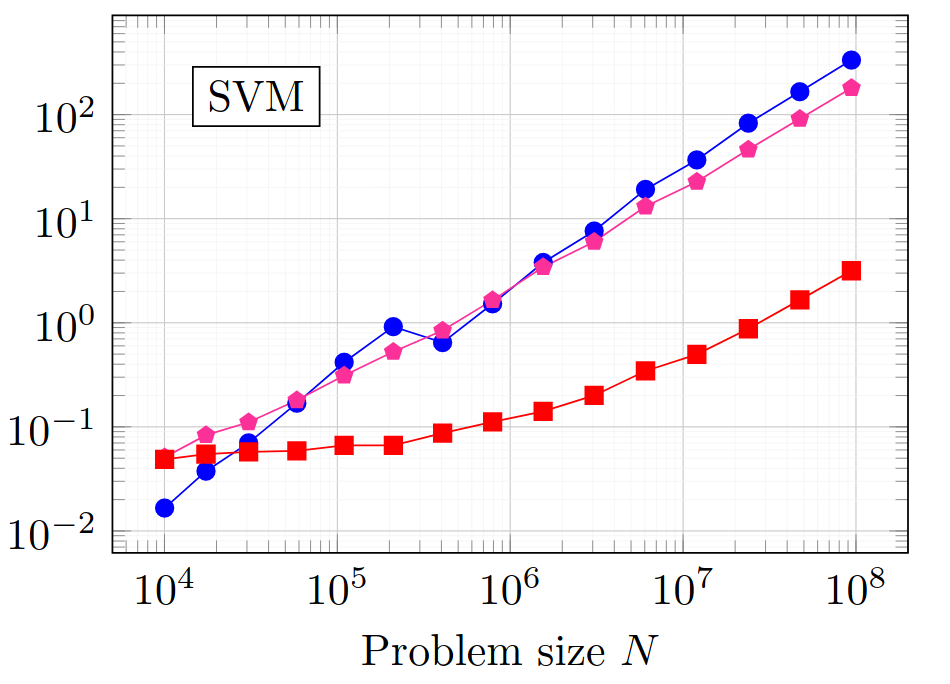
\includegraphics[scale=.25]{./media/cuosqp_results.png}
\label{fig:cuosqp_results}
\caption{This a plot replicated from \cite{cuosqp}. The red line on the right-hand graph shows the performance of the algorithm from \citep{cuosqp} in terms of runtime measured in seconds versus problem size. The blue line is the CPU implementation from \cite{osqp}. }
\end{figure}\\
They found that using a GPU implementation for SVM solving didn't give massive improvements. However the CPU implementation scales much faster than the GPU implementation as the problem size increases. Furthermore, latency between the host and target devices meant that for smaller problems, the CPU algorithm was superior to the GPU algorithm. But as the problem size increased, the overhead was overcome and the GPU achieved better performance.
\paragraph{} For our implementation, we were unable to generate problems greater than $10^4$. However, we did see similar performance improvements, our results are pictured in Fig. \ref{fig:results}. As was the case for the official implementation, we found that for small problem size, the overhead made the CPU more efficient than the GPU. But, as the problem size increased, the GPU gave superior performance. And, as the problem size increased, the GPU runtime increased at a much slower rate than the CPU runtime. 
\begin{figure}[h]
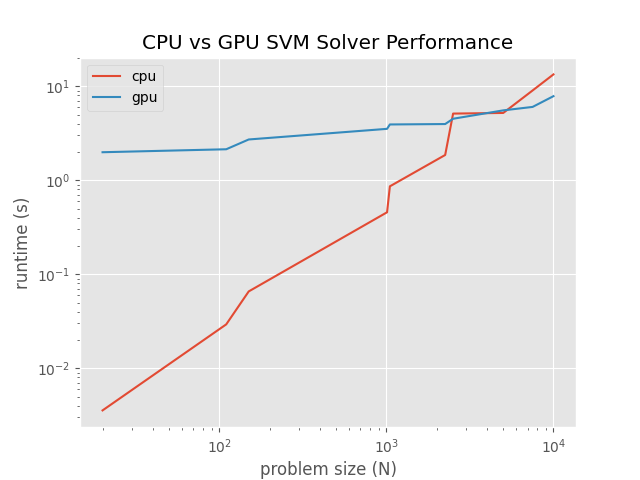
\includegraphics[scale=.6]{./media/results.png}
\label{fig:results}
\caption{This a plot of our SVM solver results. Unlike the results presented by \cite{cuosqp}, we were not able to generate problems larger than $10^4$. However, the trends in the graphs are the same. For larger problem sizes, GPU outperforms CPU, and GPU performance scales better for larger problems. These metrics were compiled by generating random SVM problems of different sizes, then averaging over several problems. All experiments were run on a Jetson Nano.}
\end{figure}\\

\section{Conclusion}

\paragraph{} In conclusion, we were able to develop our own version of a GPU implementation of ADMM for SVM classification using the \texttt{osqp} api. We also successfully verified the results from \cite{cuosqp} for small scale problems. 
\clearpage
\bibliography{bib}{}
\bibliographystyle{IEEEtran}
\clearpage
\section{Appendix A: Code}
The code is used to generate SVM classification problems \texttt{dmm.py}, the main model code. 
%\lstinputlisting[language=Python,frame=single]{./code/generate_problem.py}
\clearpage
The code below contains all of the main \texttt{CUDA} routines for the PGC algorithm.
%\lstinputlisting[language=C,frame=single]{./code/cuda_pcg.cu}
\clearpage
The code below wraps the \texttt{CUDA} functions into a \texttt{linsys} solver module specified by the \texttt{osqp} api so that we can actually solve a linear system via PCG.
%\lstinputlisting[language=C,frame=single]{../code/wrapper.py}

\end{fullwidth}

\end{document}